\documentclass[letterpaper]{article} % DO NOT CHANGE THIS
\usepackage[submission]{aaai2027}  % DO NOT CHANGE THIS
% The serif, sans-serif, and monospaced fonts are loaded automatically by
% aaai2027.sty (newtxtext, helvet, courier). DO NOT add \usepackage{times},
% \usepackage{helvet}, \usepackage{courier}, or any other font package.
\usepackage[hyphens]{url}  % DO NOT CHANGE THIS
\usepackage{graphicx} % DO NOT CHANGE THIS
\urlstyle{rm} % DO NOT CHANGE THIS
\def\UrlFont{\rm}  % DO NOT CHANGE THIS
\usepackage{natbib}  % DO NOT CHANGE THIS AND DO NOT ADD ANY OPTIONS TO IT
\usepackage{caption} % DO NOT CHANGE THIS AND DO NOT ADD ANY OPTIONS TO IT
\frenchspacing  % DO NOT CHANGE THIS
%
% These are recommended to typeset algorithms but not required. See the subsubsection on algorithms. Remove them if you don't have algorithms in your paper.
\usepackage{algorithm}
\usepackage{algorithmic}

%
% These are recommended to typeset listings but not required. See the subsubsection on listing. Remove this block if you don't have listings in your paper.
\usepackage{newfloat}
\usepackage{listings}
\DeclareCaptionStyle{ruled}{labelfont=normalfont,labelsep=colon,strut=off} % DO NOT CHANGE THIS
\lstset{%
	basicstyle={\footnotesize\ttfamily},% footnotesize acceptable for monospace
	numbers=left,numberstyle=\footnotesize,xleftmargin=2em,% show line numbers, remove this entire line if you don't want the numbers.
	aboveskip=0pt,belowskip=0pt,%
	showstringspaces=false,tabsize=2,breaklines=true}
\floatstyle{ruled}
\newfloat{listing}{tb}{lst}{}
\floatname{listing}{Listing}

%
% Recommended for better-looking tables
\usepackage{booktabs}

%
% Keep the \pdfinfo as shown here. There's no need
% for you to add the /Title and /Author tags.
\pdfinfo{
/TemplateVersion (2027.1)
}

% DISALLOWED PACKAGES
% \usepackage{authblk} -- This package is specifically forbidden
% \usepackage{balance} -- This package is specifically forbidden
% \usepackage{CJK} -- This package is specifically forbidden
% \usepackage{float} -- This package is specifically forbidden
% \usepackage{flushend} -- This package is specifically forbidden
% \usepackage{fullpage} -- This package is specifically forbidden
% \usepackage{geometry} -- This package is specifically forbidden
% \usepackage{hyperref} -- This package is specifically forbidden
% \usepackage{navigator} -- This package is specifically forbidden
% (or any other package that embeds links such as navigator or hyperref)
% \usepackage{indentfirst} -- This package is specifically forbidden
% \usepackage{layout} -- This package is specifically forbidden
% \usepackage{multicol} -- This package is specifically forbidden
% \usepackage{nameref} -- This package is specifically forbidden
% \usepackage{savetrees} -- This package is specifically forbidden
% \usepackage{setspace} -- This package is specifically forbidden
% \usepackage{stfloats} -- This package is specifically forbidden
% \usepackage{tabu} -- This package is specifically forbidden
% \usepackage{titlesec} -- This package is specifically forbidden
% \usepackage{tocbibind} -- This package is specifically forbidden
% \usepackage{ulem} -- This package is specifically forbidden
% \usepackage{wrapfig} -- This package is specifically forbidden
% DISALLOWED COMMANDS
% \nocopyright -- Your paper will not be published if you use this command
% \addtolength -- This command may not be used
% \balance -- This command may not be used
% \baselinestretch -- Your paper will not be published if you use this command
% \clearpage -- No page breaks of any kind may be used for the final version of your paper
% \columnsep -- This command may not be used
% \newpage -- No page breaks of any kind may be used for the final version of your paper
% \pagebreak -- No page breaks of any kind may be used for the final version of your paper
% \pagestyle -- This command may not be used
% \tiny -- This is not an acceptable font size.
% \vspace{- -- No negative value may be used in proximity of a caption, figure, table, section, subsection, subsubsection, or reference
% \vskip{- -- No negative value may be used to alter spacing above or below a caption, figure, table, section, subsection, subsubsection, or reference

\usepackage{amsmath}
\usepackage{amssymb}
\usepackage{amsfonts}
\usepackage{subcaption}
\usepackage{chessboard}

\setcounter{secnumdepth}{0} %May be changed to 1 or 2 if section numbers are desired.

% The file aaai2027.sty is the style file for AAAI Press
% proceedings, working notes, and technical reports.
%

% Title

% Your title must be in mixed case, not sentence case.
% That means all verbs (including short verbs like be, is, using,and go),
% nouns, adverbs, adjectives should be capitalized, including both words in hyphenated terms, while
% articles, conjunctions, and prepositions are lower case unless they
% directly follow a colon or long dash
\title{AAAI Press Anonymous Submission\\Instructions for Authors Using \LaTeX{}}
\author{
    %Authors
    % All authors must be in the same font size and format.
    Written by AAAI Press Staff\textsuperscript{\rm 1}\thanks{With help from the AAAI Publications Committee.}\\
    AAAI Style Contributions by Peter Patel Schneider,
    Sunil Issar,\\
    J. Scott Penberthy,
    George Ferguson,
    Hans Guesgen,
    Francisco Cruz\equalcontrib\corresponding,
    Marc Pujol-Gonzalez\equalcontrib\corresponding
}
\affiliations{
    %Afiliations
    \textsuperscript{\rm 1}Association for the Advancement of Artificial Intelligence\\
    % If you have multiple authors and multiple affiliations
    % use superscripts in text and roman font to identify them.
    % For example,

    % Sunil Issar\textsuperscript{\rm 2},
    % J. Scott Penberthy\textsuperscript{\rm 3},
    % George Ferguson\textsuperscript{\rm 4}\corresponding,
    % Hans Guesgen\textsuperscript{\rm 5}
    % Note that the comma should be placed after the superscript

    1101 Pennsylvania Ave, NW Suite 300\\
    Washington, DC 20004 USA\\
    % email address must be in roman text type, not monospace or sans serif
    proceedings-questions@aaai.org
%
% See more examples next
}

%Example, Single Author, ->> remove \iffalse,\fi and place them surrounding AAAI title to use it
\iffalse
\title{My Publication Title --- Single Author}
\author {
    Author Name
}
\affiliations{
    Affiliation\\
    Affiliation Line 2\\
    name@example.com
}
\fi

\iffalse
%Example, Multiple Authors, ->> remove \iffalse,\fi and place them surrounding AAAI title to use it
\title{My Publication Title --- Multiple Authors}
\author {
    % Authors
    First Author Name\textsuperscript{\rm 1,\rm 2}\equalcontrib,
    Second Author Name\textsuperscript{\rm 2}\equalcontrib,
    Third Author Name\textsuperscript{\rm 1}\corresponding
}
\affiliations {
    % Affiliations
    \textsuperscript{\rm 1}Affiliation 1\\
    \textsuperscript{\rm 2}Affiliation 2\\
    firstAuthor@affiliation1.com, secondAuthor@affilation2.com, thirdAuthor@affiliation1.com
}
\fi



\cbDefinePgfFieldStyle{masktoken}{
    \fill[gray!80] (-0.5,-0.5) rectangle (0.5,0.5);
    \node[text=white, font=\sffamily\bfseries\Large] at (0,0) {?};
}






\begin{document}

\maketitle

\begin{abstract}
    AAAI creates proceedings, working notes, and technical reports directly from electronic source furnished by the authors. To ensure that all papers in the publication have a uniform appearance, authors must adhere to the following instructions.
\end{abstract}

% Uncomment the following to link to your code, datasets, an extended version or similar.
% You must keep this block between (not within) the abstract and the main body of the paper.
% Make sure that you do not de-anonymize yourself with these links.
% \begin{links}
%     \link{Code}{https://aaai.org/example/code}
%     \link{Datasets}{https://aaai.org/example/datasets}
%     \link{Extended version}{https://aaai.org/example/extended-version}
% \end{links}

\section{Introduction}


\begin{figure*}[t]
    \begin{subfigure}[t]{0.23\textwidth}
        \centering
        \chessboard[
            setfen=6k1/7p/pPp1P1pP/P4R2/6p1/r7/4r3/1K5R w - - 0 43,
            showmover=true, % 8 / 2606
            boardfontsize=12pt
        ]
        \caption{Solution: f5b5 c6b5 b6b7, Themes: advantage, endgame, short, rook endgame}
        \label{fig:final puzzle1}
    \end{subfigure}
    \hfill
    \centering
    \begin{subfigure}[t]{0.23\textwidth}
        \centering
        \chessboard[
            setfen=r1b2k1r/2B1ppb1/p4np1/1p5p/1q3Pn1/PBN5/2P2QPP/3R1R1K w - - 1 22,
            showmover=true, % 19 / 2606
            boardfontsize=12pt
        ]
        \caption{Solution: f2d2 b4d6 c7d6, Themes: crushing, middlegame, short}
        \label{fig:final puzzle2}
    \end{subfigure}
    \hfill
    \begin{subfigure}[t]{0.23\textwidth}
        \centering
        \chessboard[
            setfen=2r1k3/4qpp1/1p2P2p/pP1Q1p2/2Np4/P1r2R2/2P3P1/7K w - - 1 34,
            showmover=true, % 21 / 2606
            boardfontsize=12pt
        ]
        \caption{Solution: e6f7 e8f8 c4e5 e7e5 d5e5, Themes: advantage, endgame, short}
        \label{fig:final puzzle3}
    \end{subfigure}
    \hfill
    \begin{subfigure}[t]{0.23\textwidth}
        \centering
        \chessboard[
            setfen=6k1/1bp1qpb1/3r1p1p/pp4P1/2BB1P1p/1P1Q1PR1/P1P1r3/1K1R4 w - - 0 23,
            showmover=true, % 88 / 2606
            boardfontsize=12pt
        ]
        \caption{Solution: g5h6 h4g3 d3g6 e7f8 h6g7 f8g7 g6g7 g8g7 c4e2, Themes: long, middlegame, advantage, kingside attack, pin}
        \label{fig:final puzzle4}
    \end{subfigure}
    \caption{A set of chess puzzles created with specific themes. White is to move first in each puzzle. The solution and the themes the generation was conditioned on are presented below the puzzles.}
    \label{fig:final puzzles}
\end{figure*}


\textcolor{red}{Edit freely, just placeholders}
The idea of machine intelligence has intrigued researchers for decades, dating back to Turing's early work on indistinguishable machine behavior \cite{turing1950computingmachineryandintelligence}. In recent years, this pursuit has culminated in the rapid rise of Large Language Models (LLMs), which might already be capable of passing standard Turing test \cite{jones2026largelanguagemodelspassastandardthreepartyturingtest}. A key benchmark for evaluating the success of these systems is creativity \cite{colton2012computationalcreativity}. However, while modern language models are capable of creative work, such as creating art, writing stories or making lyrics, they struggle with coming up with truly new and unique items \cite{wenger2026llmsarehomogenouslycreative}. To address this limitation and enhance the controllability of creative generation, we turn to chess puzzle generation, which serves as a playground for improving these qualities.

Simultaneously to the rise of autoregressive language models, diffusion models have been successfully adapted to discrete sequences and language modelling tasks. Lately, discrete diffusion models that transform random vocabulary tokens into text have become popular \cite{diffusiongemma}, as they offer some advantages compared to autoregressive models. Such models perform worse than autoregressive models thus far, however, another discrete diffusion paradigm, masked diffusion \cite{austin2021structureddenoisingdiffusionmodels,nie2025largelanguagediffusionmodels} offers comparable performance to traditional LLMs. Unlike autoregressive generation, which builds sequences token-by-token from left to right, diffusion models iteratively refine the entire sequence globally. Masked diffusion models transform a sequence of unknown mask tokens into structured text by iteratively unmasking the token sequence. This non-directional generation process offers a promising alternative for tasks that demand following strict constraints. We select a masked diffusion model for our task.

We use chess puzzle generation as a framework for improving the capabilities of language models. This domain requires the models to balance between creativity and reasoning, as chess puzzles are generally delicate. Changing even one piece on the board may entirely change the puzzle to something completely different. We take inspiration from \cite{feng2025generatingcreativechesspuzzles} and define puzzles as chess positions, which have a unique best solution, as well as are sufficiently counter-intuitive. With this definition, we observe that a notably low proportion of positions are puzzles even in the Lichess dataset \cite{lichesspuzzledatabase}. Around $1.29\%$ of the positions pass these conditions in the Lichess dataset.

To train our model for this task, we first employ supervised training on the Lichess puzzles dataset \cite{lichesspuzzledatabase}. Our model takes a list of themes as an input and is able to generate positions, which match the given theme. After supervised training, we observe that around $0.18\%$ of the positions generated by our model are valid puzzles. To improve this further, we employ reinforcement learning, as we are able to use the puzzle criteria as the reward function. We are able to improve our model to generate puzzles around $0.37\%$ of the time.

We present four main contributions from this research that build on \cite{feng2025generatingcreativechesspuzzles}. Firstly, we verify the results of \cite{feng2025generatingcreativechesspuzzles} by demonstrating the effectiveness of masked diffusion models for generating structured outputs, specifically in the context of chess puzzle generation. Secondly, we demonstrate that puzzle generation can be conditioned on specific tactical themes, which addresses a limitation in \cite{feng2025generatingcreativechesspuzzles}. Thirdly, we demonstrate that the performance of masked diffusion models can be improved through reinforcement learning, despite the difficulty of the task. This contribution builds on the reinforcement learning (RL) framework  originally designed for autoregressive LLMs in \cite{feng2025generatingcreativechesspuzzles}, which we adapt and modify for masked diffusion models. Lastly, we introduce a new auxiliary task, best move generation, and demonstrate that it can further improve puzzle generation quality. We hope that these contributions generalize to other natural language processing (NLP) tasks.

We also present example puzzles generated by our model. In Figure \ref{fig:final puzzles}, we see four different puzzles with unique themes. For each puzzle, the solution and the themes on which we conditioned the generation are in the caption. First, the puzzles were filtered so that the uniqueness and counter intuitiveness checks pass, and the actual themes present in the puzzle match the ones the generation was conditioned on. These puzzles were hand-picked based on elegance of the solution, which may reflect authors chess knowledge.








\section{Related work}
\textcolor{red}{Edit freely, just placeholders}

\paragraph{Machine intelligence and creativity}


\paragraph{Chess puzzle generation}


\paragraph{Masked diffusion models}

While autoregressive large language models (LLMs) currently dominate language modelling, discrete diffusion models have emerged as a compelling alternative \cite{nie2025largelanguagediffusionmodels,ye2025dream7bdiffusionlarge}. Unlike autoregressive generation, which generates sequences token-by-token in a causal manner, discrete diffusion models iteratively refine the entire sequence globally using bidirectional attention \cite{austin2021structureddenoisingdiffusionmodels}. This non-causal structure allows the model to leverage context from the entire input sequence simultaneously and has been shown to reduce training data memorization \cite{luo2026characterizingmemorizationdiffusionlanguage}. Furthermore, diffusion models offer variable inference-time efficiency by adjusting the number of denoising steps \cite{austin2021structureddenoisingdiffusionmodels}. However, they are computationally more expensive to pretrain to achieve comparable text quality \cite{nie2025scalingmaskeddiffusionmodels}. Some tasks, which do not have the inherent left-to-right structure of language, such as sudoku might even benefit from the approach of diffusion models, where the order of the generated tokens is not fixed \cite{Ye2025beyondautoregression}.


\paragraph{Reinforcement learning with diffusion models}


Diffusion models have computationally intractable sequence-level likelihood, which makes RL different from LLMs.

\cite{ou2025principledrldiffusionllms,zhao2025d1scalingreasoningdiffusion,wang2026d2improvingresoning,rojas2025improvingreasoningdiffusionlanguage,black2024trainingdiffusionmodelsreinforcement,fan2023dpok,SuttonAndBarto2018}



\section{Methods}
\label{sec:methods}


\subsection{Supervised training}

We begin our work by pretraining a masked diffusion model for chess puzzle generation. We follow the formalization of masked diffusion models given by \cite{shi2025simplifiedgeneralizedmaskeddiffusion}, where sequences are generated by iteratively choosing tokens from a vocabulary to replace mask tokens $[\mathtt{MASK}]$. On each step of the algorithm, the number of unmasked tokens is determined by a masking schedule. We choose to use a linear schedule $\alpha_t = 1 - t$. The probability distribution of the next token given the previous one is given by the following equation:
\begin{equation}
    p_\theta(y_s \mid y_t, x) = \text{Cat}(y_s; \bar{R}^{\mu_\theta(y_t, x)}(t, s)^\top y_t),
    \label{eq:reverse process}
\end{equation}
where $\bar{R}$ is the transition matrix defining the unmasking probabilities and Cat is the categorical distribution. Conceptually, a masked token at step $t$ is unmasked at step $s$ to a token sampled from the model's output distribution with probability $\frac{\alpha_s - \alpha_t}{1 - \alpha_t}$. Using \eqref{eq:reverse process}, we define the evidence lower bound (ELBO), which is maximized during supervised training. With the formulation of \cite{shi2025simplifiedgeneralizedmaskeddiffusion}, the ELBO is computed as a weighted sum of cross-entropy losses. For a more detailed explanation of masked diffusion models, we recommend \cite{shi2025simplifiedgeneralizedmaskeddiffusion}.

As we condition the generative process on puzzle themes, our model inputs a one-hot encoding of the themes. We choose the themes based on the Lichess puzzler project \cite{lichesspuzzler}, which implements checks for each theme. \textcolor{red}{A complete list of themes is given in the Appendix}. To represent a chess board, we use the Forsyth-Edwards notation \cite{fennotation}, which we tokenize in a similar manner as \cite{ruoss2024amortizedplanninglargescaletransformers,feng2025generatingcreativechesspuzzles}. We, however, use separate tokens to represent different concepts in the FEN. For instance, a black bishop and the concept black-to-move are given separate tokens even though they are both represented by the character b.

To evaluate how best move prediction affects the model performance, we train two different configurations on the Lichess puzzle dataset \cite{lichesspuzzledatabase}: one with a sequence length of 81 that generates both the puzzle and the best move, and another with a sequence length of 76 that only generates the puzzle. Both configurations are transformer encoders with 268M parameters, based on the 200M parameter transformer architecture from \cite{ruoss2024amortizedplanninglargescaletransformers}. In our models, the conditioning is implemented via an additional cross-attention mechanism in each transformer block, which mostly accounts for the 68M additional parameters. In total, we train the models for 2,000,000 steps. Following \cite{feng2025generatingcreativechesspuzzles}, we select the checkpoints with the lowest validation loss, which occurs at 1,000,000 steps for both models.

In addition to the two model configurations, we also experiment with block diffusion to investigate the effect of best move prediction on the puzzle quality \cite{arriola2025blockdiffusion}. With block diffusion, we split the generative process into two phases. The first phase generates the board state while artificially keeping the best move tokens masked. Only after all board tokens have been generated, is the best move sampled. We use this as a middleground between the two models, as with block diffusion, the model has learned internal representations for the best move, but is unable to use them for the generation.



% \subsection{Masked Diffusion Models}
% While autoregressive large language models (LLMs) currently dominate language modelling, discrete diffusion models have emerged as a compelling alternative \cite{nie2025largelanguagediffusionmodels,ye2025dream7bdiffusionlarge}. Unlike autoregressive generation, which generates sequences token-by-token in a causal manner, discrete diffusion models iteratively refine the entire sequence globally using bidirectional attention \cite{austin2021structureddenoisingdiffusionmodels}. This non-causal structure allows the model to leverage context from the entire input sequence simultaneously and has been shown to reduce training data memorization \cite{luo2026characterizingmemorizationdiffusionlanguage}. Furthermore, diffusion models offer variable inference-time efficiency by adjusting the number of denoising steps \cite{austin2021structureddenoisingdiffusionmodels}. However, they are computationally more expensive to pretrain to achieve comparable text quality \cite{nie2025scalingmaskeddiffusionmodels} and suffer from intractable sequence-level likelihood computation, which complicates standard reinforcement learning algorithms \cite{ou2025principledrldiffusionllms,rojas2025improvingreasoningdiffusionlanguage,zhao2025d1scalingreasoningdiffusion,wang2026d2improvingresoning}.

% In this work, we train a masked diffusion model to generate chess puzzles represented as token sequences. We follow the formalization of \cite{shi2025simplifiedgeneralizedmaskeddiffusion}, where the forward process corrupts the complete puzzle sequence $y$ by iteratively replacing tokens with a special $[\mathtt{MASK}]$ token according to a linear schedule $\alpha_t = 1 - t$ for $t \in [0, 1]$ \cite{shi2025simplifiedgeneralizedmaskeddiffusion}. The reverse process reconstructs the original tokens using a denoising network $\mu_\theta(y_t, x)$, which predicts the vocabulary distribution $V$ for each masked position given the noisy sequence $y_t$ and conditioning metadata $x$. The reverse transition probability of moving to a less masked state $s < t$ is defined as \cite{shi2025simplifiedgeneralizedmaskeddiffusion}:
% \begin{equation}
%     p_\theta(y_s \mid y_t, x) = \text{Cat}(y_s; \bar{R}^{\mu_\theta(y_t, x)}(t, s)^\top y_t)
%     \label{eq:reverse process}
% \end{equation}
% where $\bar{R}$ is the transition matrix defining the unmasking probabilities. Conceptually, a masked token at step $t$ is unmasked at step $s$ to a token sampled from the model's vocabulary distribution with probability $\frac{\alpha_s - \alpha_t}{1 - \alpha_t}$ \cite{shi2025simplifiedgeneralizedmaskeddiffusion}.

% During pretraining, we optimize the evidence lower bound (ELBO) over the target sequence $y$ given the metadata $x$ \cite{kingma2021variationaldiffusionmodels}, which corresponds to minimizing the weighted cross-entropy loss over the masked tokens \cite{shi2025simplifiedgeneralizedmaskeddiffusion}. During inference, we generate puzzles from a fully masked sequence by unmasking tokens using \eqref{eq:reverse process} via ancestral sampling. \cite{shi2025simplifiedgeneralizedmaskeddiffusion} suggest sampling from the categorical distribution using the Gumbel-max trick \cite{kool2019stochasticbeamsandwheretofindthem}. Optionally, we experiment using block diffusion for inference \cite{arriola2025blockdiffusion}, where sampling is split into two phases: the model first generates the board state with the move tokens masked, and then denoises the optimal move conditioned on that board. With block diffusion, we aim to investigate how the best move prediction capability affects the quality of the generated puzzles. For further details on masked diffusion, we recommend \cite{shi2025simplifiedgeneralizedmaskeddiffusion}.




\subsection{Denoising Diffusion Policy Optimization}
Similarly to \cite{feng2025generatingcreativechesspuzzles}, we apply reinforcement learning to optimize the pretrained model for puzzle quality metrics. For RL training, we adapt the Denoising Diffusion Policy Optimization (DDPO) algorithm \cite{black2024trainingdiffusionmodelsreinforcement}. Although DDPO was originally developed for image-generation models, we adapt it to masked diffusion models by using the transition probabilities from the reverse process as the policy $\pi_\theta(a_t \mid s_t, x) = p_\theta(a_t \mid s_t, x)$. Additionally, we adapt the group relative advantage calculation from GRPO \cite{shao2024deepseekmathpushinglimitsmathematical}, which is originally not part of DDPO. DDPO acts in a step-wise Markov Decision Process (MDP), where the states are defined to be a partially masked token sequences $s_t$. The actions $a_t$ correspond to sampling a new partially masked token sequence with the transitions being deterministic. The reward is given at the end of the trajectory for the full generated sequence and propagated through the trajectory via discounting.

As shown by \cite{feng2025generatingcreativechesspuzzles}, a pure reward maximization procedure suffers from entropy collapse. Like their work, we employ diversity filtering mechanisms alongside an entropy bonus and a KL divergence penalty to prevent entropy collapse and ensure the realism of the puzzles. However, we optimize these penalties directly via gradient descent by incorporating them into the loss function. Using this setup, we seek to maximize the following objective:
\begin{equation}
    \mathcal{J}(\theta) = L(\theta) - \beta \mathbb{E}_t\left[\mathbb{KL}(\pi_\theta \parallel \pi_{\text{ref}})\right] + \gamma \mathbb{E}_t\left[H(\pi_\theta)\right]
\end{equation}
where $L(\theta) = \mathbb{E}_t [ \min(\rho_t \hat{A}_t, \text{clip}(\rho_t, 1-\epsilon, 1+\epsilon)\hat{A}_t) ]$ is the proximal policy optimization (PPO) objective \cite{schulman2017proximalpolicyoptimizationalgorithms}, and $\mathbb{E}_t\left[\mathbb{KL}(\pi_\theta \parallel \pi_{\text{ref}})\right]$ and $\mathbb{E}_t\left[H(\pi_\theta)\right]$ are the expected step-wise KL divergence and the entropy, respectively. The advantages $\hat{A}_t$ are computed and normalized group-wise using an unbiased Monte Carlo estimate proposed by \cite{kool2019unbiasedbaseline}.




\subsection{Defining chess puzzles}
Following \citeauthor{feng2025generatingcreativechesspuzzles}, we define a chess position to be a puzzle if it passes legality, uniqueness \eqref{eq:uniqueness_condition}, and counter-intuitiveness criteria \eqref{eq:counter-intuitiveness_condition}. We attempt to define and implement the metrics in the same way as \cite{feng2025generatingcreativechesspuzzles}, but minor unknown differences remain.

\paragraph{Uniqueness}
A position $s$ is unique if the winning chances after the best move are considerably larger than those after the second best move \cite{lichesspuzzler,feng2025generatingcreativechesspuzzles}.
\begin{equation}
    \mathbb{I}_{\text{uni}}(s) = w(a_{\text{best}} \mid s) - w(a_{\text{second}} \mid s) > \tau_{\text{uni}},
    \label{eq:uniqueness_condition}
\end{equation}
where $w(a \mid s)$ yields the winning probability of move $a$ in position $s$ \cite{Lichessaccuracymetric} and $\tau_{\text{uni}} = 0.5$.

\paragraph{Counter-intuitiveness}
The counter-intuitvity value of a position is defined as follows \cite{feng2025generatingcreativechesspuzzles}:
\begin{equation}
    r_{\text{cnt}}(s) = 0.8 \cdot \frac{d_{\text{cp}} - 1}{50} - 0.1 \cdot \frac{v_{\text{captured}}}{9}
    \label{eq:counter-intuitiveness_condition}
\end{equation}
where $d_{\text{cp}} \le 50$ is the critical depth at which Stockfish first discovers the best move, and $v_{\text{captured}}$ is the value of the potentially captured piece. A position is considered counte-intuitive if $r_{\text{cnt}}(s) > \tau_{\text{cnt}} = 0.1$.

\paragraph{Reward function}

We defined the RL reward function $R(s)$ as:
\begin{equation}
    R(s) = \begin{cases}
        -2                                 & \text{if } \neg\mathbb{I}_{\text{legal}}(s)                                                                  \\
        \max(10\cdot r_{\text{cnt}}(s), 0) & \text{if } \mathbb{I}_{\text{legal}}(s) \cdot \mathbb{I}_{\text{filter}}(s) \cdot \mathbb{I}_{\text{uni}}(s) \\
        0                                  & \text{otherwise}
    \end{cases}
    \label{eq:reward function}
\end{equation}
where $\mathbb{I}_{\text{filter}}(s) = \mathbb{I}_{\text{diversity}}(s) \cdot \mathbb{I}_{\text{pieces}}(s) \cdot \mathbb{I}_{\text{theme}}(s)$. $\mathbb{I}_{\text{pieces}}(s)$ filters out positions in which the piece count of some piece exceeds that of the starting position, and $\mathbb{I}_{\text{theme}}(s)$ indicates that the generated puzzle adheres the requested themes. \textcolor{red}{The actual condition is provided in the Appendix}. The diversity indicator factorizes as $\mathbb{I}_{\text{diversity}}(s) = \mathbb{I}_{\text{entropy}}(s) \cdot \mathbb{I}_{\text{intra}}(s) \cdot \mathbb{I}_{\text{inter}}(s)$, where $\mathbb{I}_{\text{entropy}}(s)$ filters out low-entropy generations, $\mathbb{I}_{\text{intra}}(s)$ filters out positions that are too similar to each other in the same batch and $\mathbb{I}_{\text{inter}}(s)$ filters out positions that are too similar to positions in previous batches. Both intra- and inter-batch distances are computed using the Levenshtein distance \cite{li2007normalizedlevenshteindistance} over the FEN and the principal variation (PV). A position passes the conditions if the minimum distance to all other positions is greater than a threshold. For more details, we direct the reader to \cite{feng2025generatingcreativechesspuzzles}, as apart from the theme condition and the exact form of the reward function, our diversity filtering setup is very similar to theirs.

% \paragraph{Diversity Filtering}
% To prevent the model from collapsing to a single position, we use normalized Levenshtein distance metrics to penalize similarity between generated samples:
% \begin{align}
%     d_{\text{fen}}(s, s') & = \text{lev}(\text{fen}(s), \text{fen}(s'))                               \
%     d_{\text{pv}}(s, s')  & = \frac{\text{lev}(\text{pv}(s), \text{pv}(s'))}{\max(|pv(s)|, |pv(s')|)}
% \end{align}
% where $\text{fen}(s)$ represents the board FEN sequence (excluding counters) and $\text{pv}(s)$ represents the principal variation.
% The intra-batch filter $\mathbb{I}_{\text{intra}}(s)$ is set to zero if the board or PV distance to the closest item in the batch falls below thresholds $\tau_{\text{fen}}$ and $\tau_{\text{pv}}$, respectively.
% Similarly, the inter-batch filter $\mathbb{I}_{\text{inter}}(s)$ compares the generated position against a replay buffer of previous generations.





\section{Experimental evaluation}
\label{sec:experiments}

Our experimental evaluation is structured as follows. We first analyze how best move prediction affects the puzzle generation process. We also compare our model to the ones trained by \cite{feng2025generatingcreativechesspuzzles}. Second, we evaluate the reinforcement learning phase. Finally, we present how conditioning affects the generation, specifically during the RL phase.

\begin{table*}[t]
    \centering
    \caption{Puzzle quality metrics for different model configurations. All models were sampled with a temperature 1.0 and 256 denoising steps for 1,000,000 positions each. The errors represent the 95\% standard errors.}
    \label{tab:metrics}
    \begin{tabular}{llccccc}
        \toprule
        Training                            & Best move                & Legal (\%)                & Unique (\%)              & Counter-Intuitive (\%)   & Puzzle (\%)              & Theme (\%)       \\
        \midrule
        Supervised                          & Yes                      & $98.95 \pm 0.05$          & $28.75 \pm 0.20$         & $0.61 \pm 0.02$          & $0.18 \pm 0.02$          & $86.27 \pm 0.19$ \\
        Supervised                          & Block                    & $98.97 \pm 0.04$          & $27.08 \pm 0.19$         & $0.63 \pm 0.02$          & $0.17 \pm 0.02$          & $85.53 \pm 0.18$ \\
        Supervised                          & No                       & $98.97 \pm 0.02$          & $25.30 \pm 0.09$         & $0.63 \pm 0.01$          & $0.16 \pm 0.01$          & $84.23 \pm 0.08$ \\
        RL                                  & Yes                      & $99.87 \pm 0.01$          & $25.28 \pm 0.09$         & $1.45 \pm 0.01$          & $0.37 \pm 0.01$          & $78.72 \pm 0.08$ \\
        \midrule
        \multicolumn{2}{l}{Lichess Puzzles} & \textbf{100.0} $\pm$ 0.0 & \textbf{83.58} $\pm$ 0.23 & \textbf{1.55} $\pm$ 0.07 & \textbf{1.29} $\pm$ 0.07 & \textbf{100.0} $\pm$ 0.0                    \\
        \bottomrule
    \end{tabular}
\end{table*}

\begin{table*}[t]
    \centering
    \caption{Self-distance and Lichess-distance metrics after supervised training and RL. Metrics are computed over positions passing the uniqueness filter. We align the number of positions with \cite{feng2025generatingcreativechesspuzzles} and use 100k samples for Lichess-distances and 40k samples for the self-distances.}
    \label{tab:distances}
    \begin{tabular}{llcccc}
        \toprule
        Training                            & Best move & Board (Self) & Board (Lichess) & PV (Self) & PV (Lichess) \\
        \midrule
        Supervised                          & Yes       & 11.55        & 11.16           & 0.87      & 0.89         \\
        Supervised                          & Block     & 11.50        & 11.13           & 0.87      & 0.89         \\
        Supervised                          & No        & 11.50        & 11.16           & 0.86      & 0.89         \\
        RL                                  & Yes       & 15.02        & 14.35           & 0.86      & 0.95         \\
        \midrule
        \multicolumn{2}{l}{Lichess Puzzles} & 11.88     & —            & 0.95            & —                        \\
        \bottomrule
    \end{tabular}
\end{table*}

% \subsection{Supervised training}
\subsection{Best move prediction improves puzzle metrics}
Table~\ref{tab:metrics} summarizes the puzzle metrics of the models trained with supervised training. We find that simultaneously generating the best move alongside the board state leads to measurable improvements in both uniqueness and theme match rates compared to generating the board alone or predicting the best move with block diffusion. Although the confidence intervals for the counter-intuitiveness and puzzle rates overlap across configurations, the model with joint best-move generation achieves the highest estimate for the final puzzle rate (0.18\%). Across all supervised configurations, the theme match rate remains remarkably high, exceeding 84\% for positions with unique solutions. This indicates that the model successfully aligns its generations with the requested conditioning in the vast majority of cases, reflecting a solid grasp of varied tactical concepts.

To quantify the novelty and diversity of the generated positions, we utilize the distance metrics summarized in Table~\ref{tab:distances}. For the baseline Lichess puzzle dataset, the board distance is 11.88, which corresponds to a difference of roughly 12 distinct board elements between a puzzle and the most similar other position. The Lichess dataset exhibits a baseline PV distance of 0.95, representing a high diversity of solutions where the start or target squares of the moves typically differ by at least one rank or file. As shown in Table~\ref{tab:distances}, all three supervised configurations closely preserve these distances. The board self-distances are only slightly lower than that of the original Lichess dataset, while the PV self-distance remains also quite similar. Furthermore, the board and PV distances to the Lichess dataset itself are high are also similar, which indicates that the distribution of generated positions is similar to the lichess dataset distribution. Importantly, the choice of the best-move generation strategy has virtually no impact on these diversity metrics, demonstrating that coupling chess understanding with the generation process to improve puzzle quality does not compromise diversity.




\subsection{Reinforcement learning}
\begin{figure}[h]
    \centering
    \chessboard[
        setfen=r4k2/1Q3ppp/1n6/8/2p5/5P2/3q2PP/4R2K w - - 2 39,
        showmover=true,
        boardfontsize=12pt
    ]
    \caption{An example of a generated puzzle after the model collapse. White is able to force a checmate in three: b7e7 f8g8 e7e8 a8e8 e1e8.}
    \label{fig:RL model collapse}
\end{figure}

\begin{figure*}[t]
    \centering
    \begin{subfigure}[t]{0.24\textwidth}
        \centering
        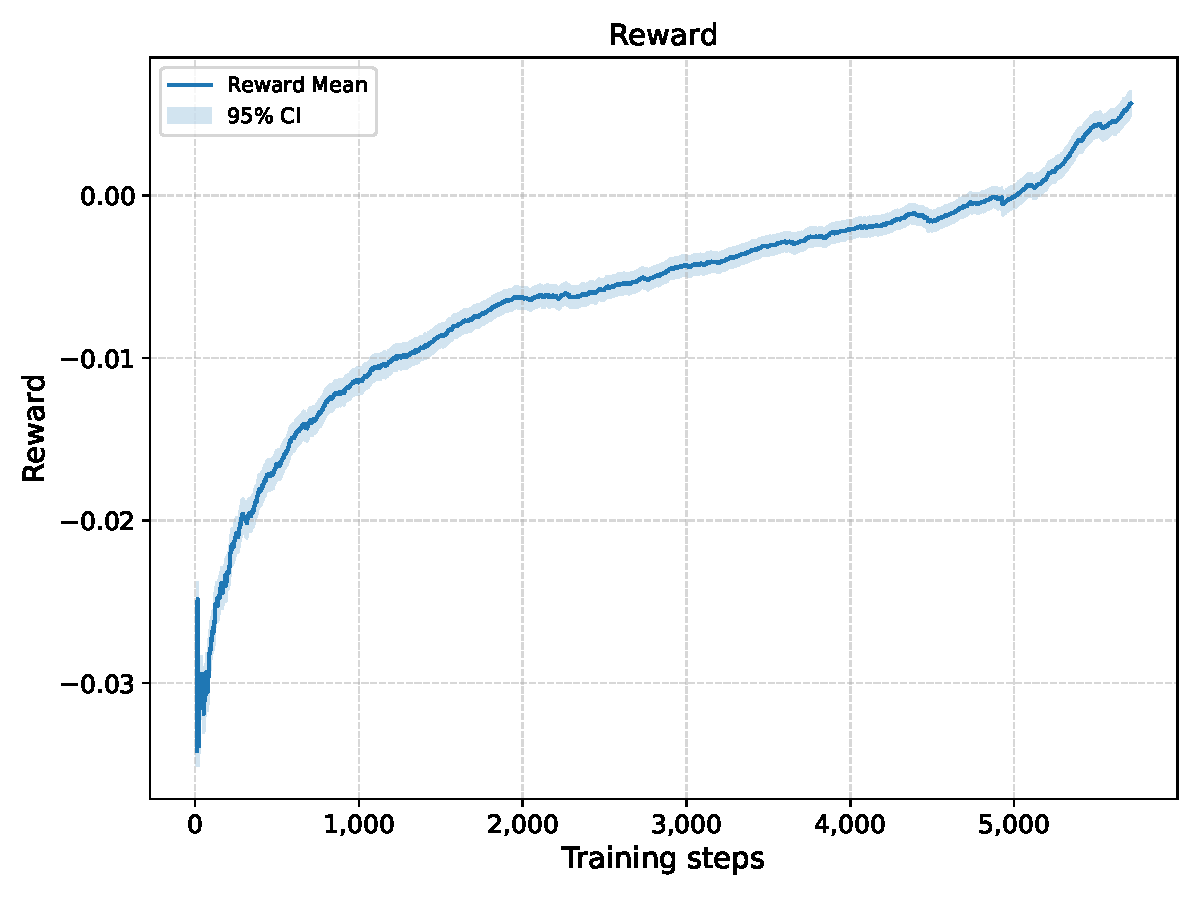
\includegraphics[width=\textwidth]{Figures/rl_training_progress/good_run/Reward.pdf}
        \caption{Reward}
        \label{fig:rl_reward}
    \end{subfigure}
    \hfill
    \begin{subfigure}[t]{0.24\textwidth}
        \centering
        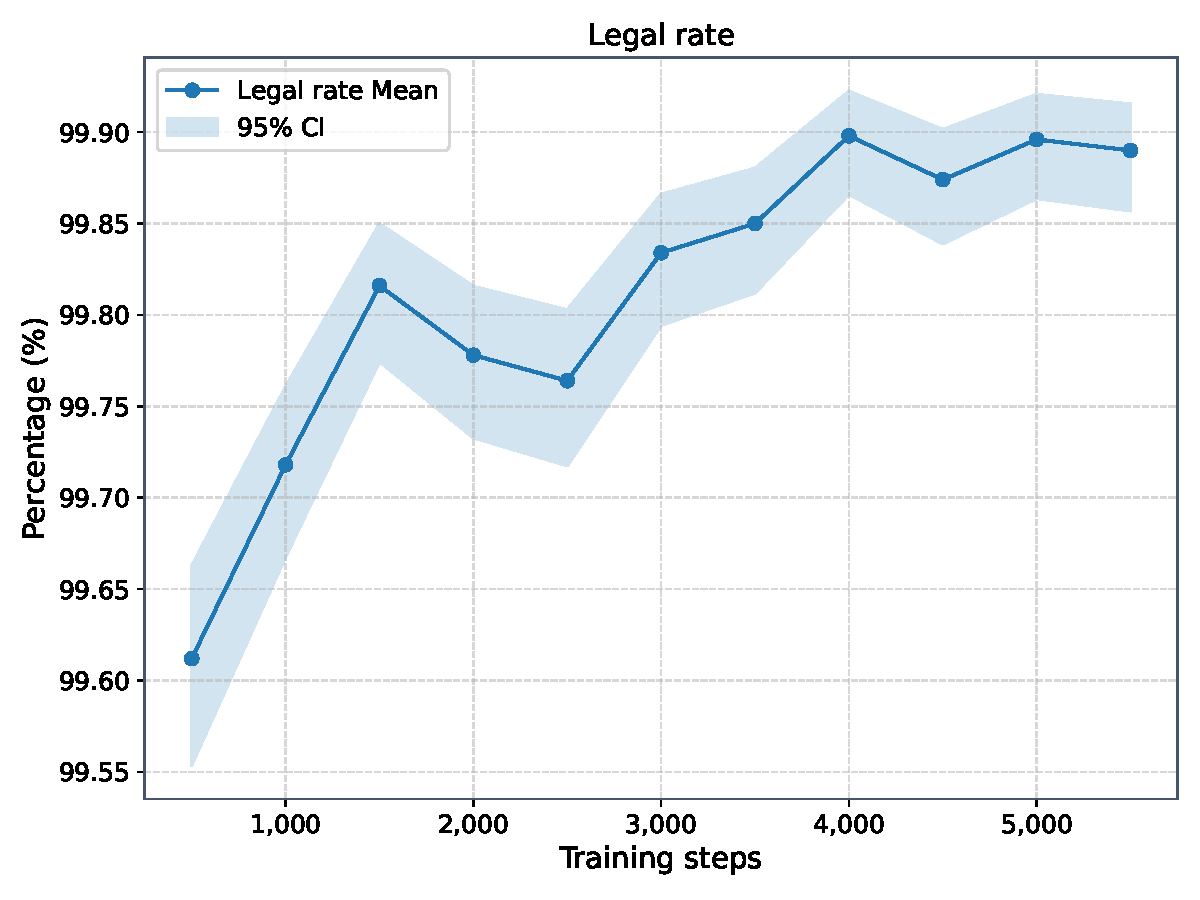
\includegraphics[width=\textwidth]{Figures/rl_training_progress/good_run/Legal_rate.pdf}
        \caption{Legal rate}
        \label{fig:rl_legal_rate}
    \end{subfigure}
    \hfill
    \begin{subfigure}[t]{0.24\textwidth}
        \centering
        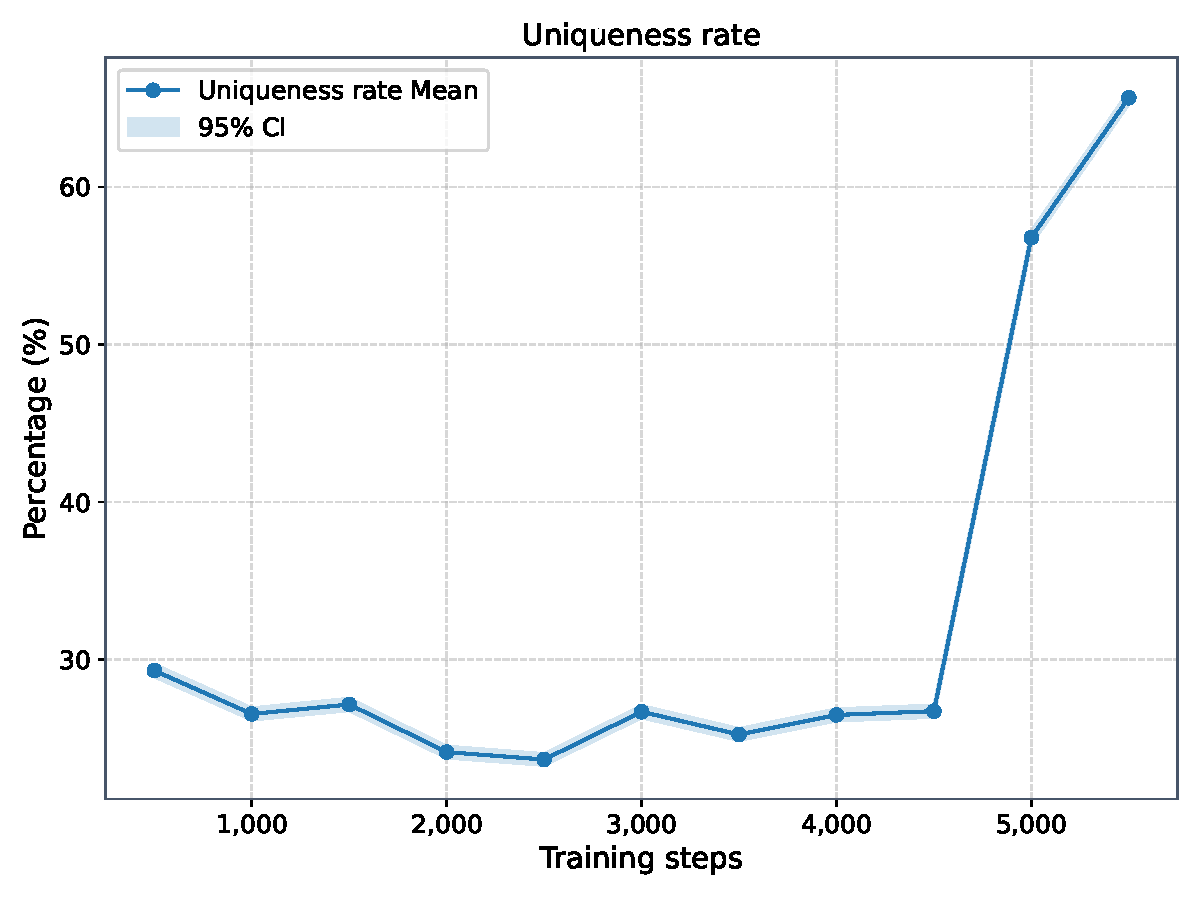
\includegraphics[width=\textwidth]{Figures/rl_training_progress/good_run/Uniqueness_rate.pdf}
        \caption{Uniqueness rate}
        \label{fig:rl_uniqueness}
    \end{subfigure}
    \hfill
    \begin{subfigure}[t]{0.24\textwidth}
        \centering
        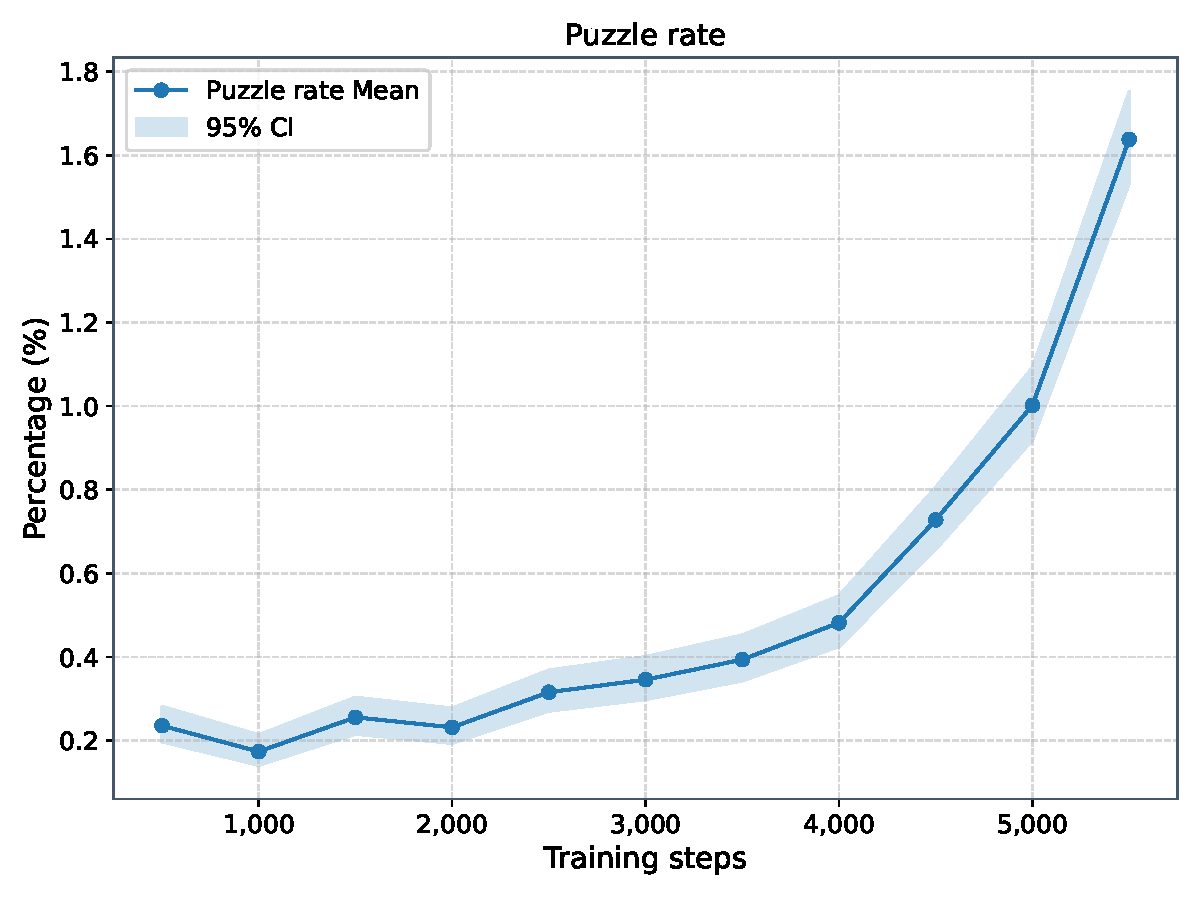
\includegraphics[width=\textwidth]{Figures/rl_training_progress/good_run/Puzzle_rate.pdf}
        \caption{Puzzle rate}
        \label{fig:rl_puzzle_rate}
    \end{subfigure}

    \vspace{0.2cm}

    \begin{subfigure}[t]{0.24\textwidth}
        \centering
        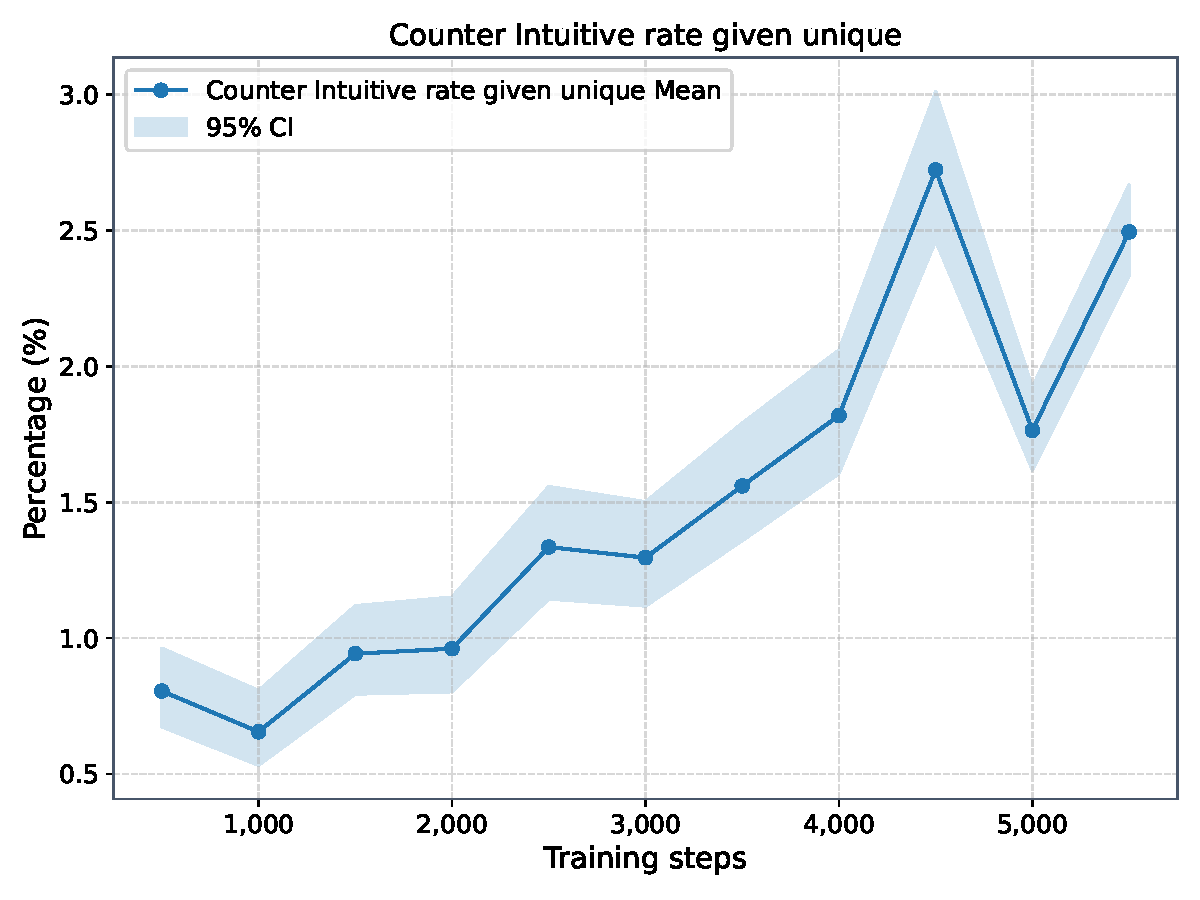
\includegraphics[width=\textwidth]{Figures/rl_training_progress/good_run/Counter_Intuitive_rate_given_unique.pdf}
        \caption{Counter-intuitive rate}
        \label{fig:rl_counter_intuitive}
    \end{subfigure}
    \hfill
    \begin{subfigure}[t]{0.24\textwidth}
        \centering
        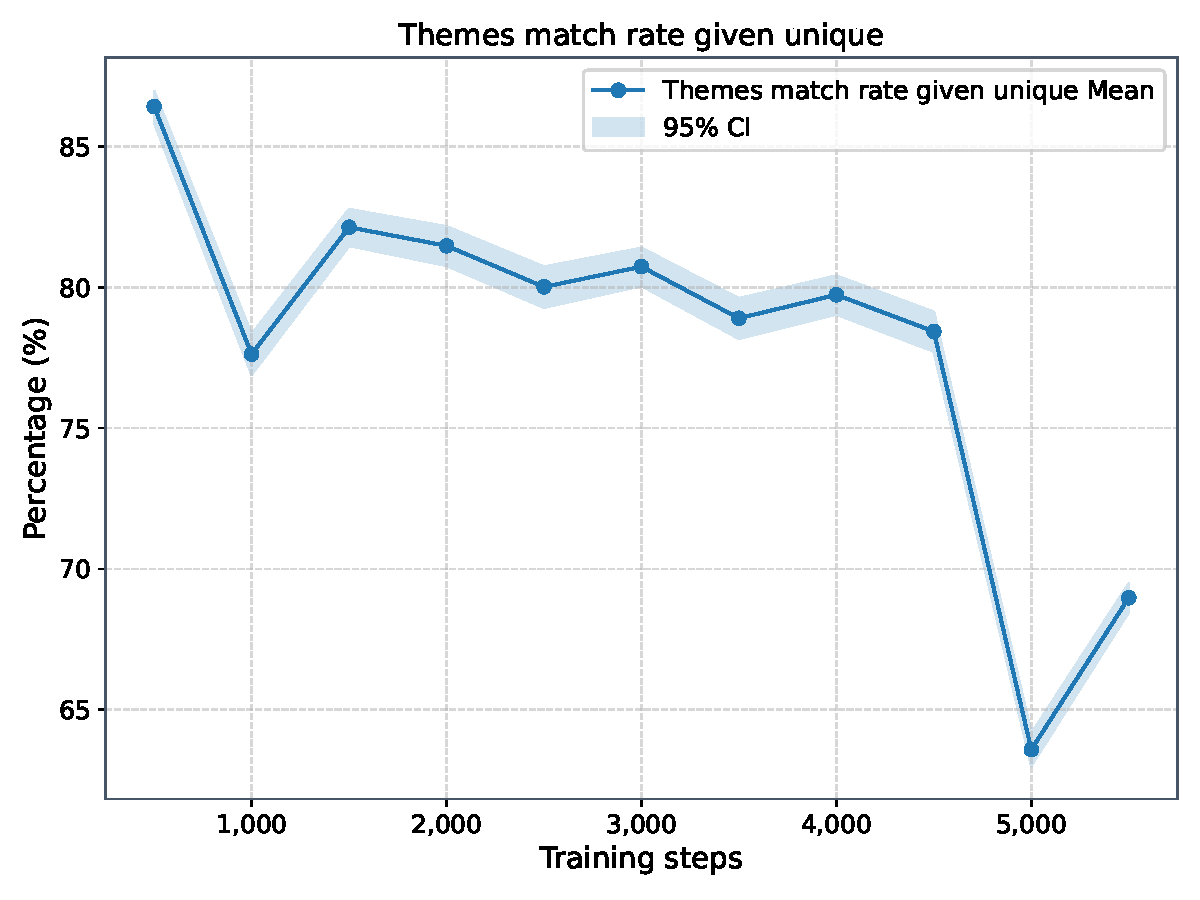
\includegraphics[width=\textwidth]{Figures/rl_training_progress/good_run/Themes_match_rate_given_unique.pdf}
        \caption{Theme match rate}
        \label{fig:rl_themes}
    \end{subfigure}
    \hfill
    \begin{subfigure}[t]{0.24\textwidth}
        \centering
        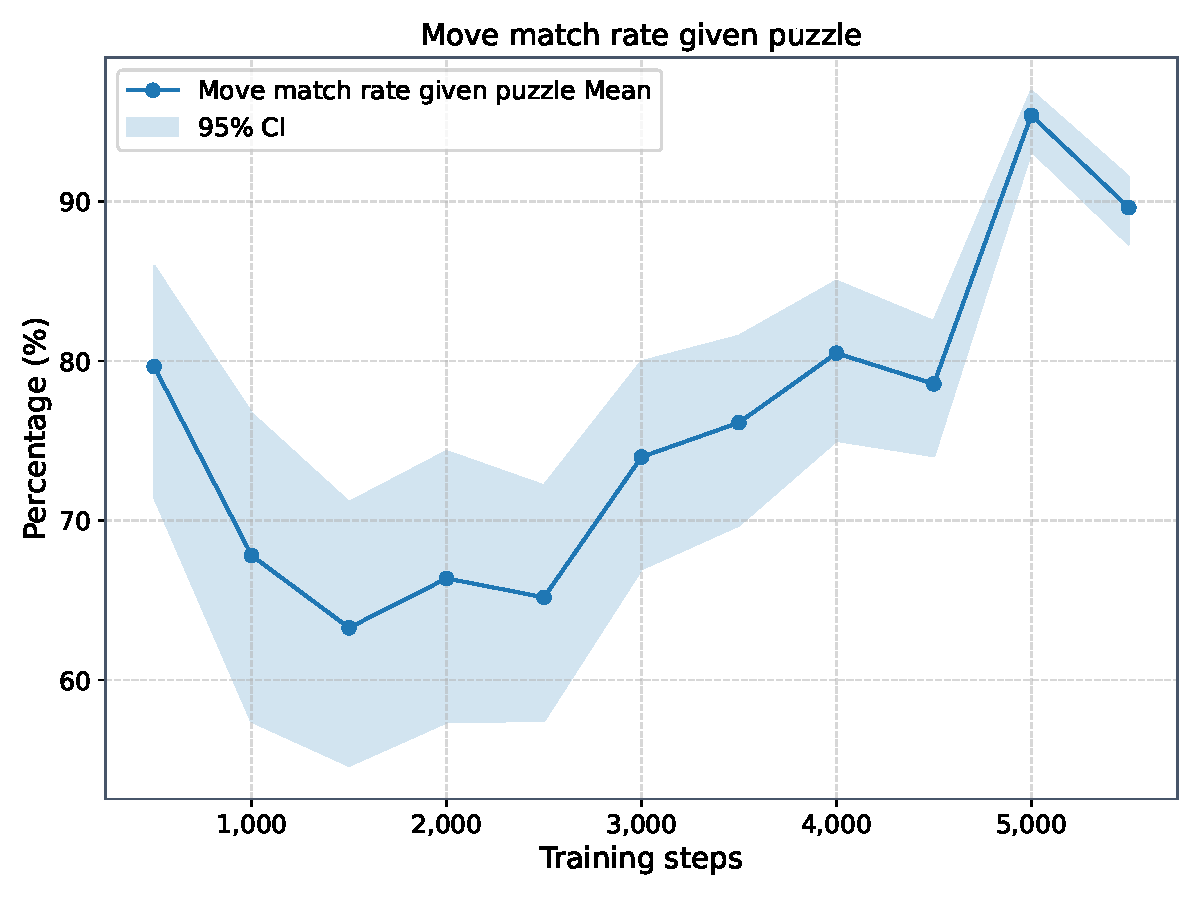
\includegraphics[width=\textwidth]{Figures/rl_training_progress/good_run/Move_match_rate_given_puzzle.pdf}
        \caption{Move match rate}
        \label{fig:rl_move_match}
    \end{subfigure}
    \hfill
    \begin{subfigure}[t]{0.24\textwidth}
        \centering
        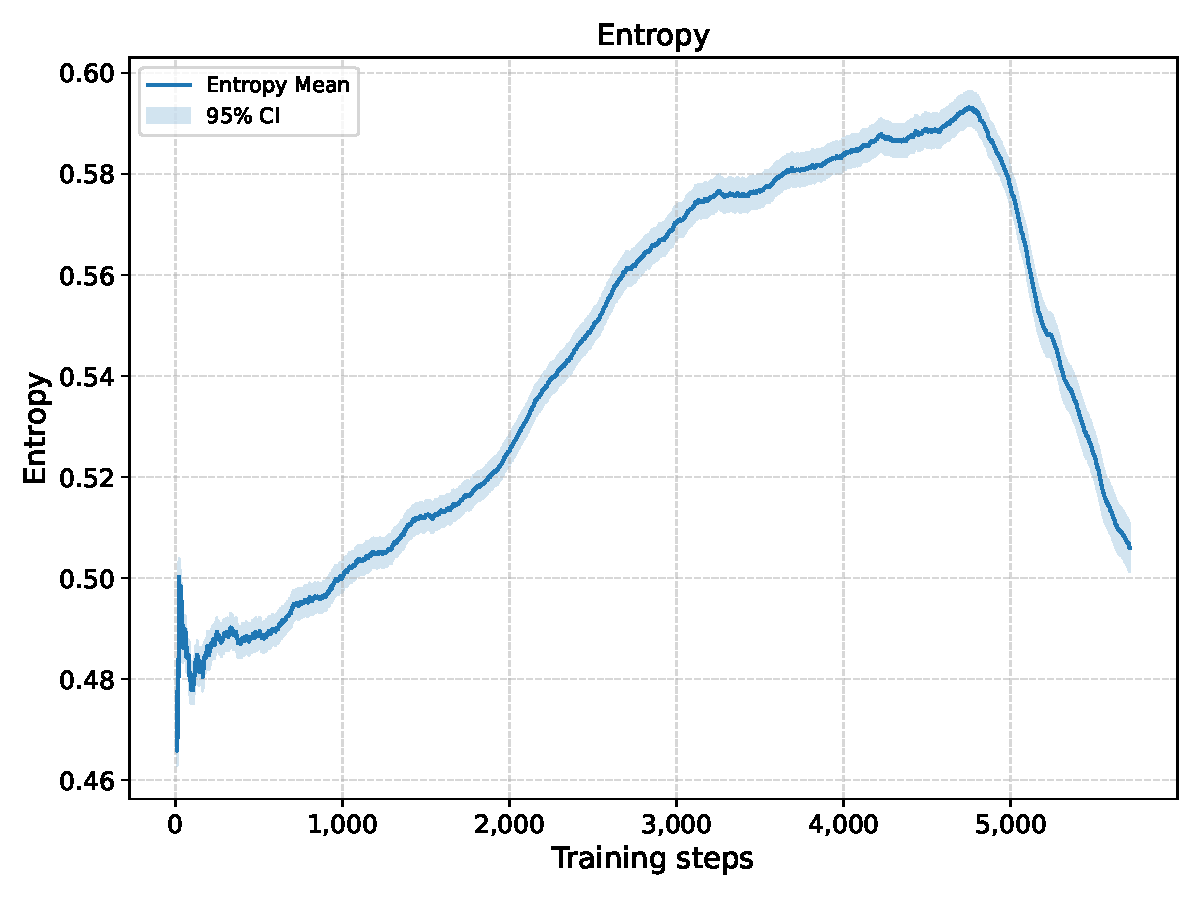
\includegraphics[width=\textwidth]{Figures/rl_training_progress/good_run/Entropy.pdf}
        \caption{Entropy}
        \label{fig:rl_entropy}
    \end{subfigure}

    \vspace{0.2cm}

    \begin{subfigure}[t]{0.24\textwidth}
        \centering
        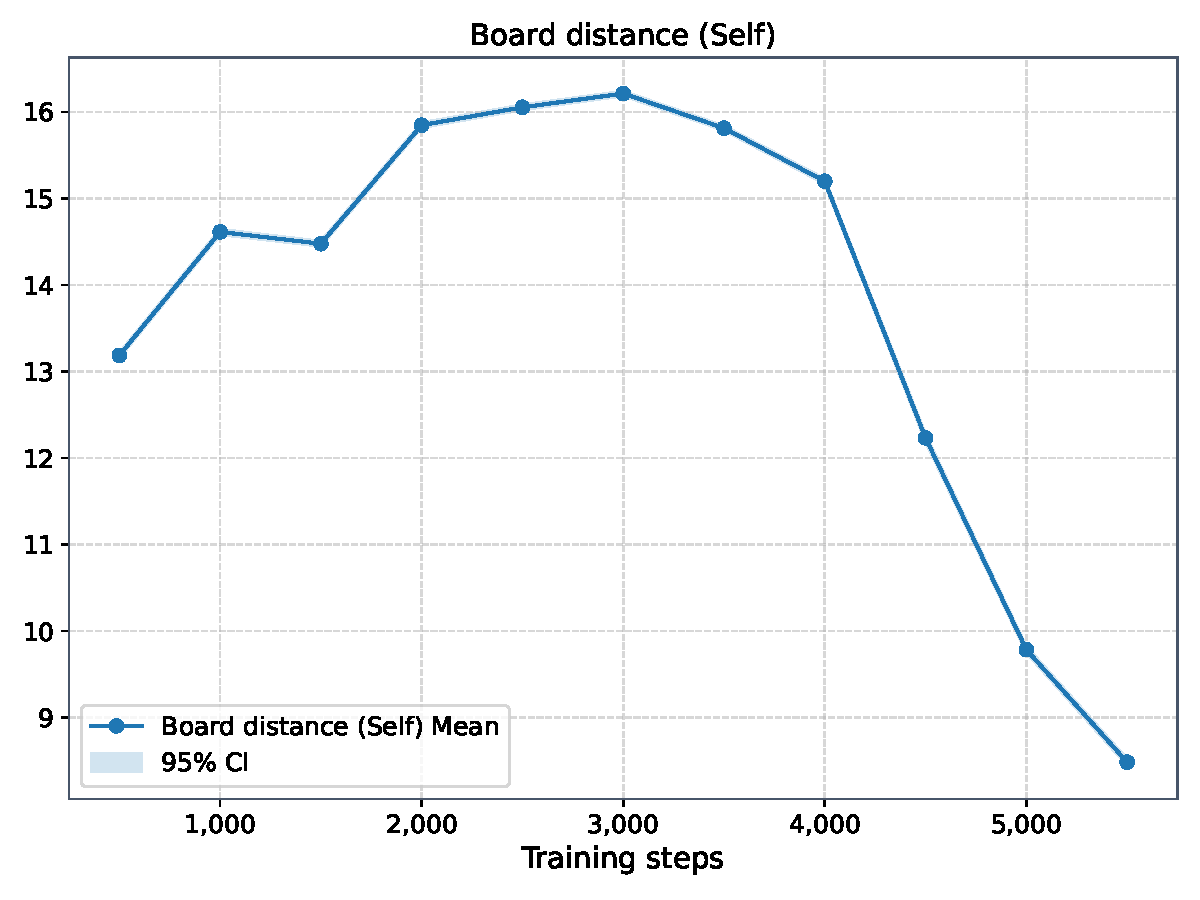
\includegraphics[width=\textwidth]{Figures/rl_training_progress/good_run/self_distance_board.pdf}
        \caption{Board distance (Self)}
        \label{fig:rl_self_board}
    \end{subfigure}
    \hfill
    \begin{subfigure}[t]{0.24\textwidth}
        \centering
        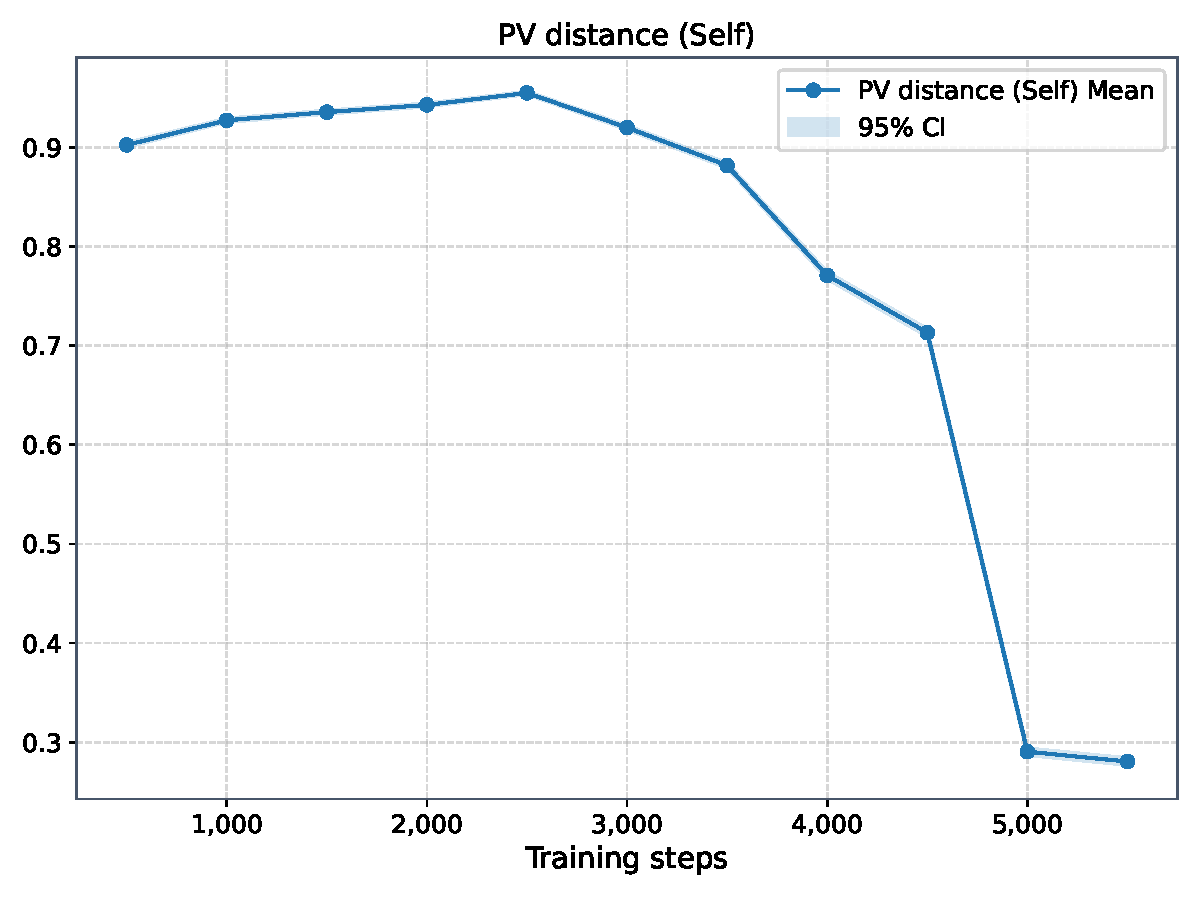
\includegraphics[width=\textwidth]{Figures/rl_training_progress/good_run/self_distance_pv.pdf}
        \caption{PV distance (Self)}
        \label{fig:rl_self_pv}
    \end{subfigure}
    \hfill
    \begin{subfigure}[t]{0.24\textwidth}
        \centering
        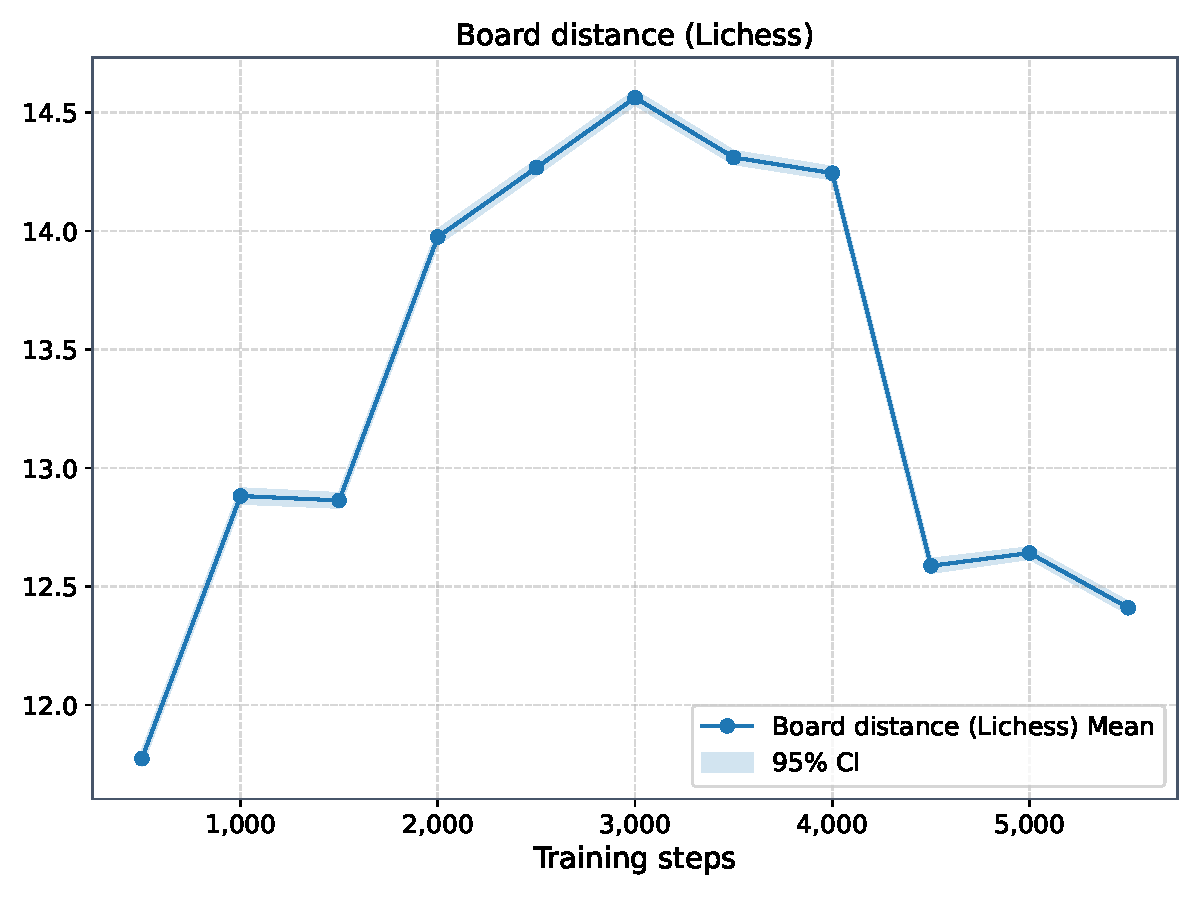
\includegraphics[width=\textwidth]{Figures/rl_training_progress/good_run/lichess_distance_board.pdf}
        \caption{Board distance (Lichess)}
        \label{fig:rl_lichess_board}
    \end{subfigure}
    \hfill
    \begin{subfigure}[t]{0.24\textwidth}
        \centering
        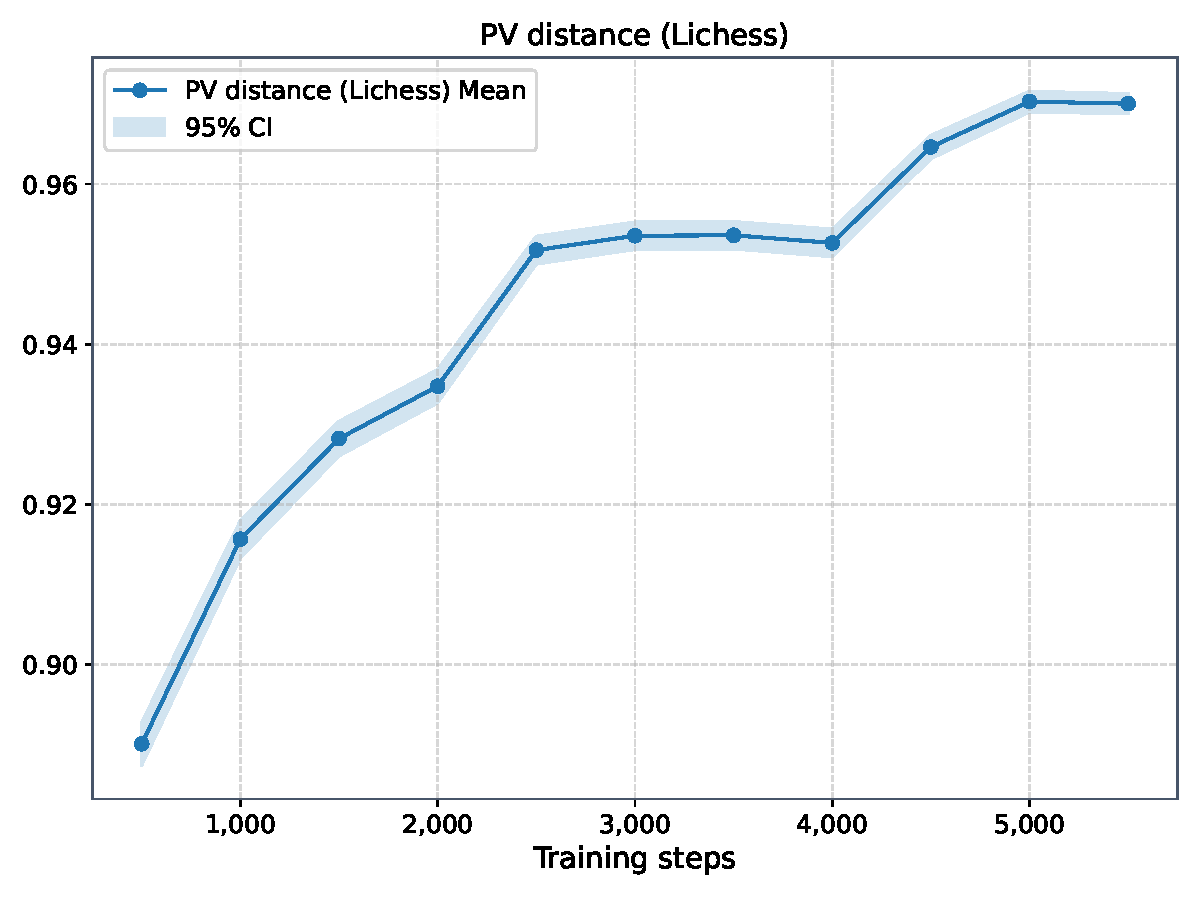
\includegraphics[width=\textwidth]{Figures/rl_training_progress/good_run/lichess_distance_pv.pdf}
        \caption{PV distance (Lichess)}
        \label{fig:rl_lichess_pv}
    \end{subfigure}
    \caption{Training progress during reinforcement learning. Model collapse occurs after approximately 4,500 steps, characterized by a sudden drop in distances. Shaded areas represent 95\% standard errors.}
    \label{fig:rl_training_progress}
\end{figure*}


For reinforcement learning, we initialize the policy from the supervised checkpoint trained with joint best-move prediction, as it achieved the highest baseline puzzle rate (0.18\%). We fine-tune this model using the DDPO framework, incorporating the diversity mechanisms we described previously.

In Figure~\ref{fig:rl_training_progress}, we present the progression of our RL run. Figures~\ref{fig:rl_reward}-\ref{fig:rl_move_match} showcase the evolution of the key performance metrics, whereas the rest of the plots concern the diversity of the generated positions. We observe that the initial improvement in the reward comes mainly from the improved legal rate. During training, the proportion of illegal positions decreases by an order of magnitude from around 1.0\% to around 0.1\%. The second metric that is improved is the counter-intuitive rate. The counter-intuitive rate for unique positions approximately doubles from under 1\% to over 2\%. The increased counter-intuitive rate also yields improvements in the puzzle rate, which improves from around 0.2\% to over 0.4\%. Lastly, we see a small decrease in the theme match rate and a small increase in the move match rate, despite not explicitly training for the best move.

For most of the RL training, the uniqueness rate stays approximately constant, however, after 4,500 training steps, the uniqueness rate rapidly increases. This sudden increase, however, is not a result of model getting better, but instead results from model collapse. As seen in Figures \ref{fig:rl_self_board}-\ref{fig:rl_lichess_board}, the distance metrics initially increase, but after around 3,000 training steps, start to decrease. As novelty is an important success metric for our model, we select the checkpoint at 3,500 steps, which still has high diversity. Interestingly, the PV distance to the Lichess dataset in \ref{fig:rl_lichess_pv} never starts to decrease suggesting that the model has found a position, which yields high rewards, but is not present in the Lichess dataset. In fact, when manually observing the generated puzzles after the model collapse, we see that the model begins to generate positions like the one in \ref{fig:RL model collapse}. Interestingly, two such positions are not immediately ruled out by the current diversity filtering procedure, as the exact positioning of the White queen and the rook are not important for the solution.

% Overall, we attempt many different things to remedy this model collapse. The position, which the last position collapses to is a backrank checkmate with a queen sacrifice.

Table~\ref{tab:metrics} presents the final puzzle metrics for the RL model at step 3,500. As seen with the training curves, we observe improvements in the legal and counter-intuitiveness rate, while see a slight decrease in uniqueness and theme match rates. Notably, although the uniqueness rate is slightly lower than in the base model, the puzzle rate is over twice as high, which is driven by the counter-intuitiveness rate. This observation is consistant with \cite{feng2025generatingcreativechesspuzzles}. In Table~\ref{tab:distances}, we see that the RL training significantly improved the novelty of the generated puzzles. While the PV self distance remains approximately constant at 0.86, the remaining distance metrics improve significantly. \textcolor{red}{Compare metrics to \cite{feng2025generatingcreativechesspuzzles} when able to compute the metrics.} Nonetheless, the overall yield of unique, counter-intuitive, and theme-compliant puzzles increases from 0.12\% to 0.26\%.





\subsection{Thematic conditioning allows for manual control}

\begin{figure*}[t]
    \centering
    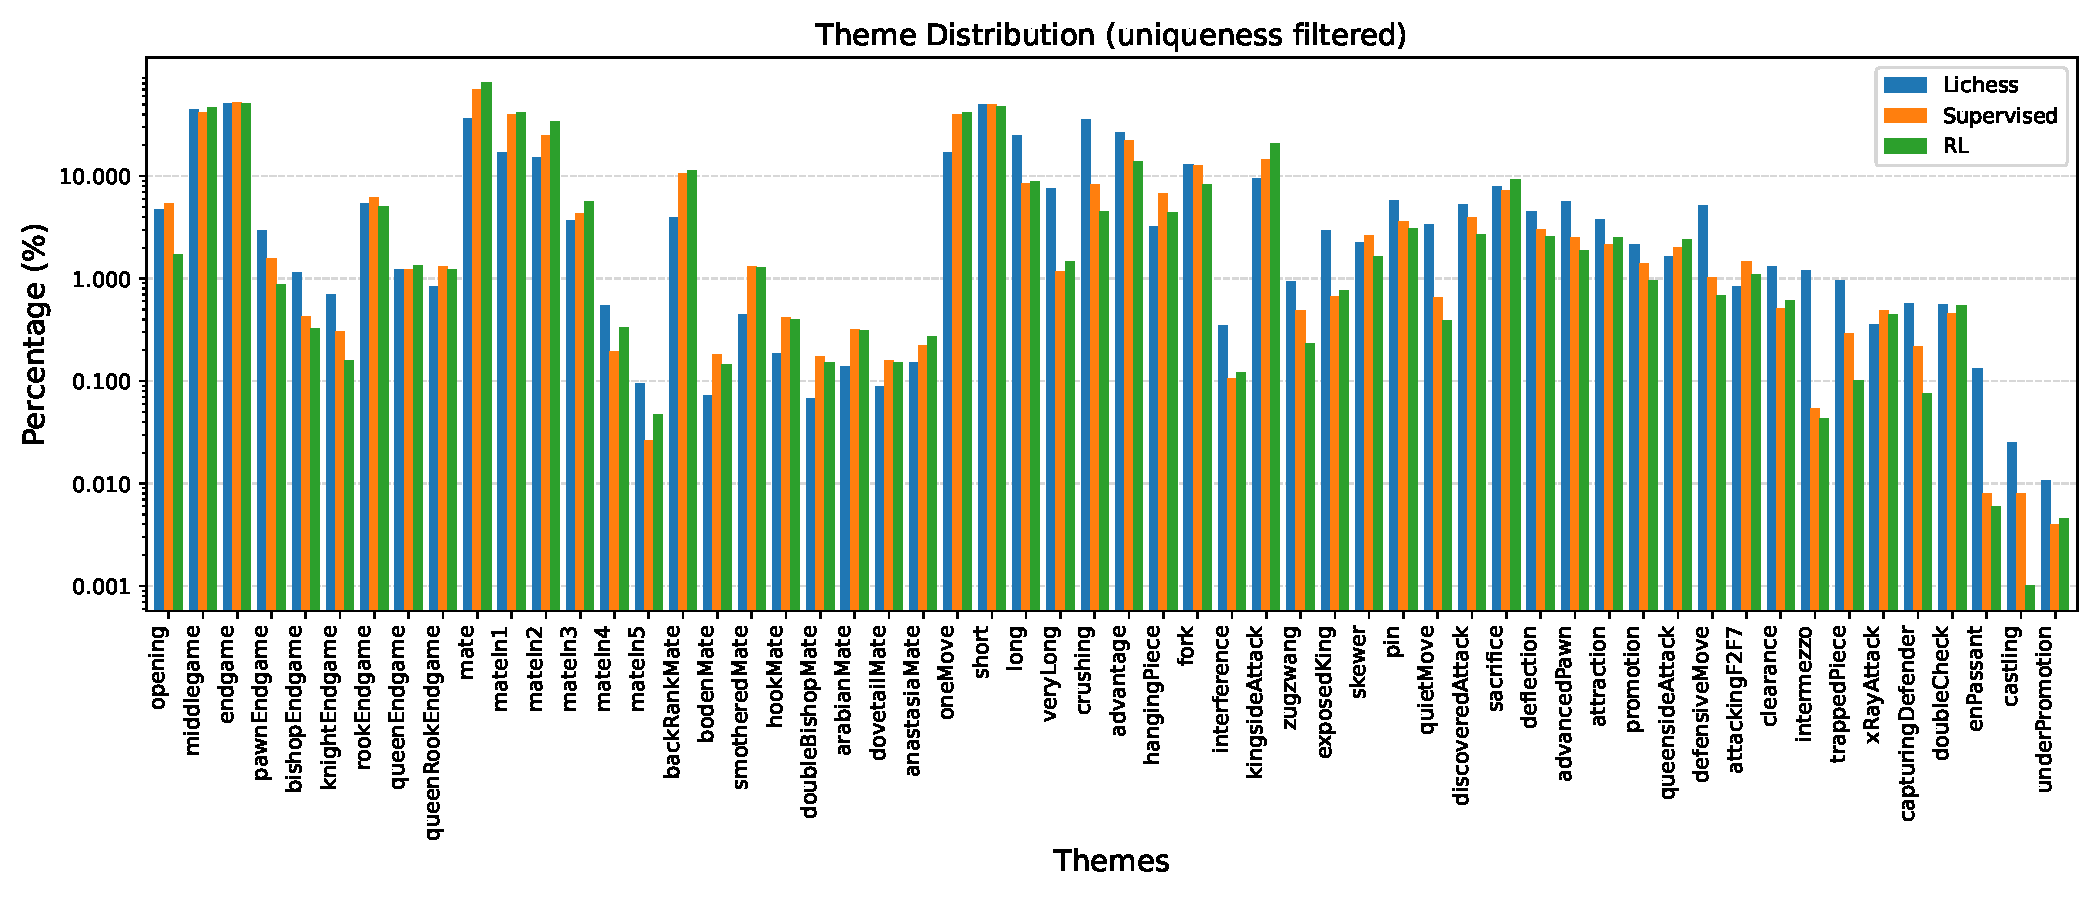
\includegraphics[width=\textwidth]{Figures/other/theme_distribution.pdf}
    \caption{The distribution of themes for the Lichess puzzles dataset, our supervised model and the final RL model. All positions are first filtered for positions with a unique solutions and the percentages are computed accross the filtered dataset.}
    \label{fig:theme_dist}
\end{figure*}

% A major advantage of our conditional generation approach compared to \cite{feng2025generatingcreativechesspuzzles} is that our setup allows for manual control of the generated puzzles. This makes our model practically more interesting, as users can practise specific themes they struggle with.

% Another advantage of our model is that conditioning and training on tactical themes allows us to retain full diversity of themes post-RL. In contrast, unconditioned models \cite{feng2025generatingcreativechesspuzzles} tend to prioritize longer and more difficult puzzles, which are usually more counter-intuitive, and suppress easier ones, as they are rewarded more during RL. In Figure~\ref{fig:theme_dist} we plot the distribution of themes for the Lichess dataset, as well as our two chosen checkpoints after supervised training and RL respectively. We observe that both the supervised model and the final RL model retain the full diversity of themes well. In particular, themes like \textit{mate-in-one} or \textit{one move} are not forgotten, even though they are practically never counter intuitive (\textcolor{red}{include the other figure in the appendix.}) and hence almost always get zero rewards.

A key contribution of our conditional generation approach is that it enables manual control over the generated puzzles. While unconditioned models, such as that by \cite{feng2025generatingcreativechesspuzzles}, generate creative puzzles at random, they do not allow users to specify which tactics they want to practice. By conditioning our model on specific themes, we make the generator practically more useful, allowing users to generate targeted practice material for positions they struggle with.

Furthermore, conditioning the generation process is crucial for retaining the full diversity of chess tactics post-reinforcement learning. Because short or simple tactics (such as \textit{one-move} or \textit{mate-in-one} puzzles) are almost never counter-intuitive, a global reward naturally suppresses them in favor of longer, more complex configurations. In contrast, our RL setup enforces theme matching via the reward function (Equation~\ref{eq:reward function}), ensuring that the model is only rewarded if the generated puzzle satisfies the requested conditioning. Additionally, the advantages are computed over groups of same conditioning, which forces the policy to maximize puzzle quality within the context of the requested theme, rather than globally converging to the more difficult themes.

Figure~\ref{fig:theme_dist} illustrates the distribution of tactical themes across the original Lichess dataset, our supervised baseline, and the final RL model. Both of our models successfully preserve the full spectrum of themes. In particular, themes like \textit{mate-in-one} are successfully retained, despite the fact that they are practically never counter-intuitive as shown in \textcolor{red}{Figure~\ref{fig:ci_over_themes}} and would otherwise receive zero reward.





% 2. Render the board
% \chessboard[
%     setfen=r1bqkbnr/pppp1ppp/2n5/4p3/4P3/8/PPPP1PPP/RNBQKBNR w KQkq - 0 1,
%     pgfstyle=masktoken,
%     markfields={f3, g3, h3, f4, g4, h4, f5, g5, h5}
% ]





\section{Conclusions and discussion}




% \section*{Acknowledgments}
% AAAI is especially grateful to Peter Patel Schneider for his work in implementing the original aaai.sty file, liberally using the ideas of other style hackers, including Barbara Beeton. We also acknowledge with thanks the work of George Ferguson for his guide to using the style and BibTeX files --- which has been incorporated into this document --- and Hans Guesgen, who provided several timely modifications, as well as the many others who have, from time to time, sent in suggestions on improvements to the AAAI style. We are especially grateful to Francisco Cruz, Marc Pujol-Gonzalez, and Mico Loretan for the improvements to the Bib\TeX{} and \LaTeX{} files made in 2020.

% The preparation of the \LaTeX{} and Bib\TeX{} files that implement these instructions was supported by Schlumberger Palo Alto Research, AT\&T Bell Laboratories, Morgan Kaufmann Publishers, The Live Oak Press, LLC, and AAAI Press. Bibliography style changes were added by Sunil Issar. \verb+\+pubnote was added by J. Scott Penberthy. George Ferguson added support for printing the AAAI copyright slug. Additional changes to aaai2027.sty and aaai2027.bst have been made by Francisco Cruz, Marc Pujol-Gonzalez, and Mico Loretan.

% \bigskip
% \noindent Thank you for reading these instructions carefully. We look forward to receiving your electronic files!

\bibliography{aaai2027}

% Check whether the conference requires a reproducibility checklist to be included in the paper.
% If so, you can uncomment the following line and ajust the path to include it.
\input{ReproducibilityChecklist.tex}







% \appendix

% \section{Additional results}

% \begin{figure}[t]
%     \centering
%     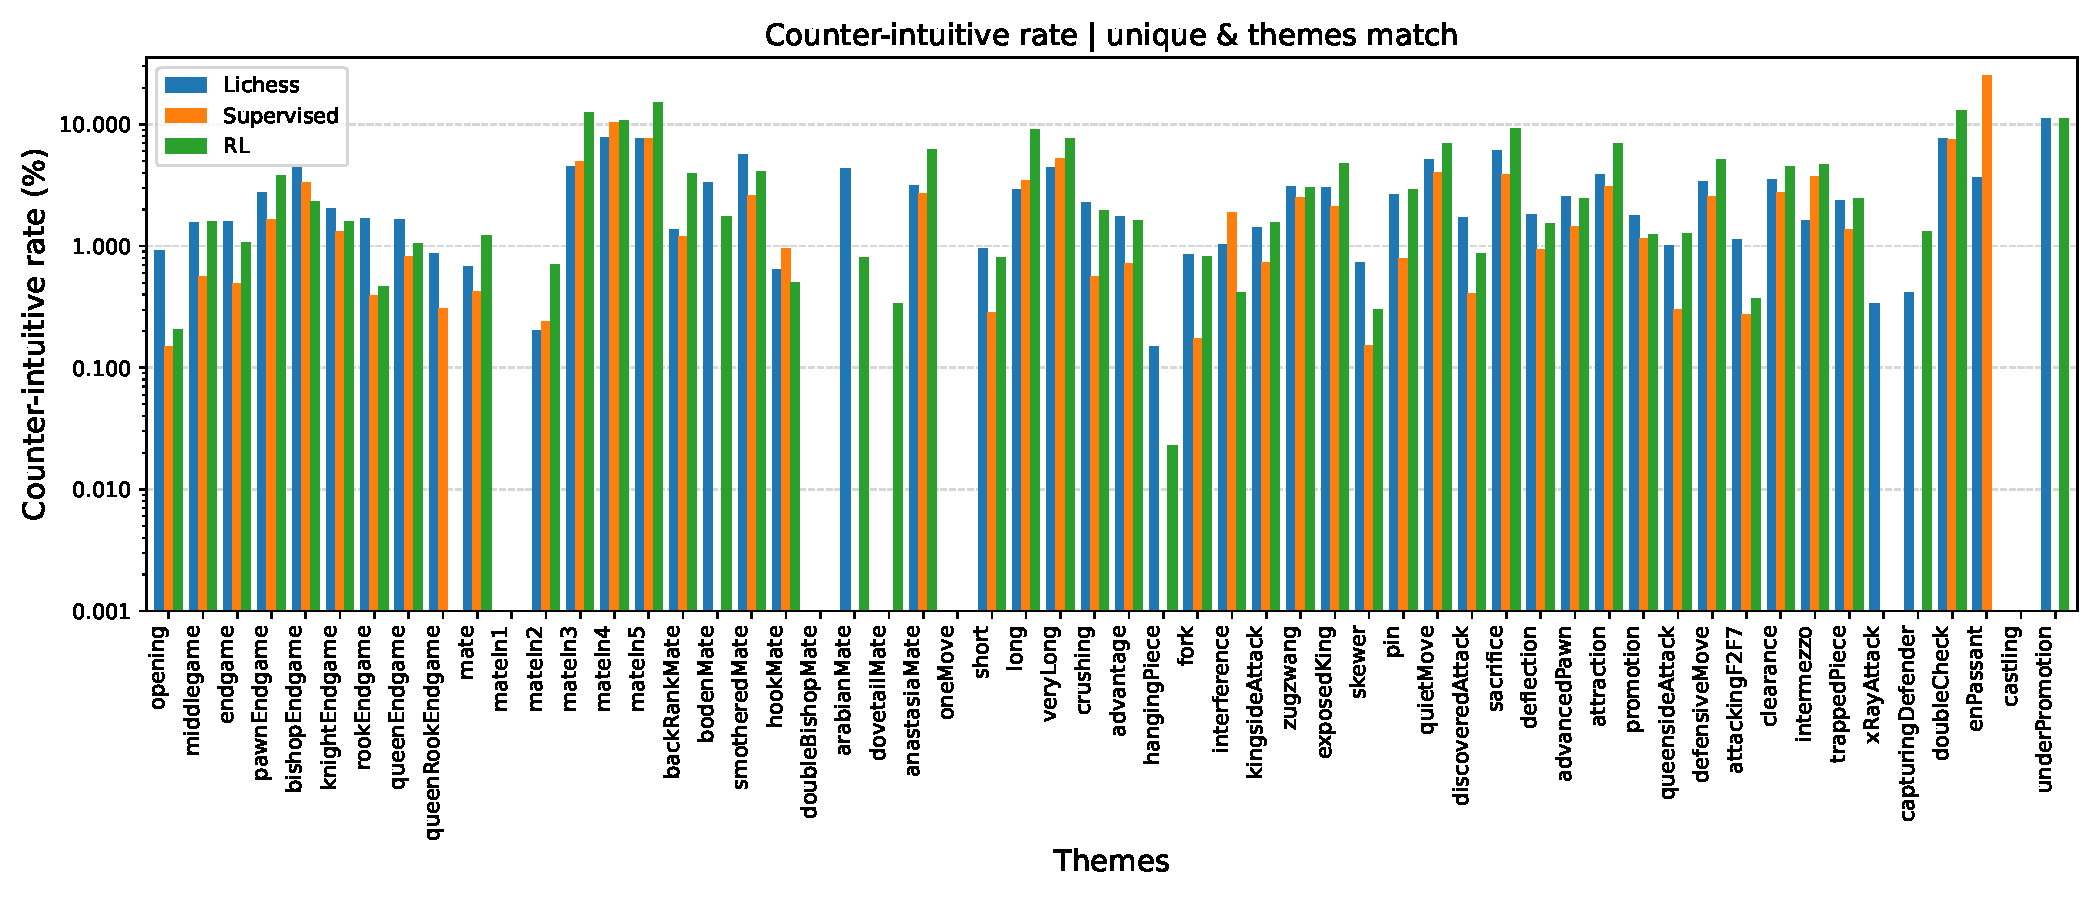
\includegraphics[width=\textwidth]{Figures/other/ci_distribution_over_themes.pdf}
%     \caption{The counter-intuitive rate for the Lichess puzzles dataset, our supervised model and the final model across all themes.}
%     \label{fig:ci_over_themes}
% \end{figure}




\end{document}
